%%%%%%%%%%%%%%%%%%%%%%%%%%%%%%%%%%%%%%%%%
% Friedrich M. Grabner - 01220997
% Masters Project Report
%%%%%%%%%%%%%%%%%%%%%%%%%%%%%%%%%%%%%%%%%

%----------------------------------------------------------------------------------------
%	PACKAGES AND DOCUMENT CONFIGURATIONS
%----------------------------------------------------------------------------------------

\documentclass{beamer}
\usepackage{graphicx} % Required for the inclusion of images
\usepackage{multicol}
\usepackage{listings}
\graphicspath{{./images/}}

\lstset{language=xml,
	tabsize=3,
    %frame=lines,
    %caption=Test,
    %label=code:sample,
    frame=shadowbox,
    rulesepcolor=\color{gray},
    xleftmargin=20pt,
    framexleftmargin=15pt,
    keywordstyle=\color{blue}\bf,
    stringstyle=\color{red},
    numbers=left,
    numberstyle=\tiny,
    numbersep=5pt,
    breaklines=true,
    showstringspaces=false,
    basicstyle=\ttfamily,
    emph={food,name,price},emphstyle={\color{magenta}}}

\setbeamertemplate{navigation symbols}{}
\usetheme{Singapore}
\beamersetuncovermixins{\opaqueness<1>{25}}{\opaqueness<2->{15}}

%----------------------------------------------------------------------------------------
%	BEGIN DOCUMENT
%----------------------------------------------------------------------------------------
\begin{document}
\setbeamertemplate{footline}[text line]{\parbox{\linewidth}{\vspace*{-8pt}\centering Imperial College London}
}
\title{\huge{HPC on the Cloud}} 
\author{Author: Friedrich Grabner\\
Supervisor: Dr C. Cantwell}
\date{\today} 

\begin{frame}
\titlepage
\end{frame}

%----------------------------------------------------------------------------------------
%	INTRODUCTION
%----------------------------------------------------------------------------------------
\section{Introduction} 
\begin{frame}\frametitle{Introduction}
\textbf{Context:}
\begin{itemize}
\item Advancements in computing power has increased the feasibility of using high-order numerical methods to solve complex engineering problems
\item Availability to IaaS systems has allowed those outside large institutions to gain access to high performance computing
\end{itemize}
\vspace{.5cm}
\textbf{\color{red}{Problem:}}
\begin{itemize}
\item Nevertheless most people still prefer to use low-order commercial software, on personal hardware
\end{itemize}
\end{frame}

\begin{frame}\frametitle{Introduction}
\textbf{Why do people prefer commercial codes?}
\vspace{.5cm}
\begin{itemize}
\item Complex and daunting interface of open-source softwares
\item High-level of expertise required to understand how to run properly run a simulation. (numerical methods, submitting jobs, post-processing)
\item Inadequate user support in open-source projects
\end{itemize}
\end{frame}

\begin{frame}\frametitle{Aims and Objectives}
\textbf{Aim:} Build a web-based GUI that generates robust input XML files for Nektar++'s incompressible flow solver.
\newline
\newline
\textbf{Objectives:}
\small
\begin{enumerate}
\item Map parameter space of incompressible flow solver in Nektar++
\item Understand and detail the constraints between parameters
\item Develop TemPSS transform templates that instantiate all parameters
\item Represent parameters and constraints within an intuitive interface
\item Perform a beta testing of the interface with Nektar++ users
\item Benchmark TemPSS using a selection of representative testcases
\end{enumerate}
\end{frame}

%----------------------------------------------------------------------------------------
%	NEKKL0UD AND TEMPSS
%----------------------------------------------------------------------------------------
\section{Nekkloud and TemPSS} 
\begin{frame}\frametitle{Nekkloud}
\begin{itemize}
\item  Nekkloud is a web based platform through which the Nektar++ solvers can be launched
\item Nekkloud streamlines the running of simulations through access to IaaS systems
\end{itemize}
\centering
\vspace{3pt}
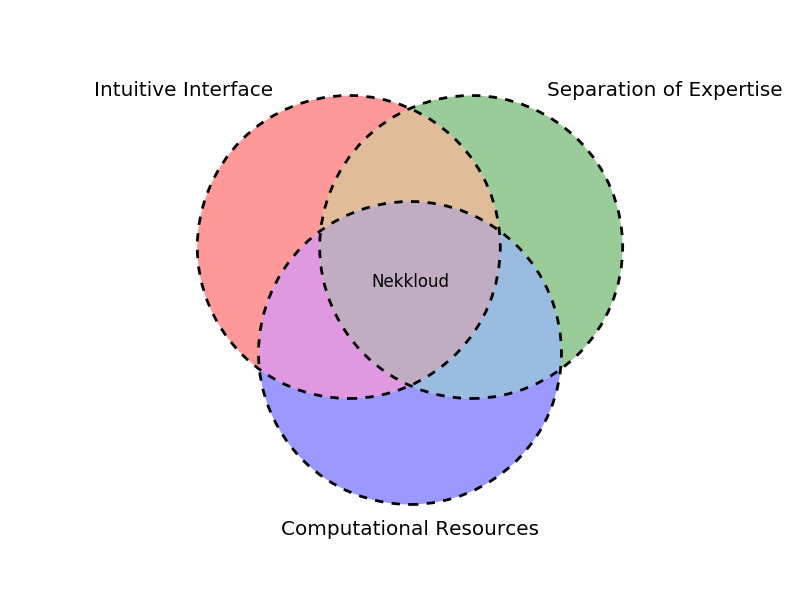
\includegraphics[width=.75\linewidth,  clip=true, trim = 0cm 0cm 0cm 2cm]{venn_diagram}
\end{frame}

\begin{frame}\frametitle{\textbf{Tem}plates and \textbf{P}rofiles for \textbf{S}cientific \textbf{S}oftware - \textbf{TemPSS}}
 
\begin{itemize}
\item Integrated into Nekkloud
\item Java based web environment hosting the user interface for Nektar++
\item Key components:  \begin{enumerate}\vspace{.25cm} \item Templates - displays parameter space of solver \item Profiles - instatiations of templates\end{enumerate}\vspace{.25cm}
\item Templates are defined by XML schema
\item Profiles can be saved and shared with other users of Nekkloud/TemPSS
\end{itemize}
\vspace{.5cm}
\centering\textbf{ \href{http://localhost:8080/tempss/profiles/}{\beamergotobutton{TemPSS Interface}}}
\end{frame}

%----------------------------------------------------------------------------------------
%	DEVELOPING THE INTERFACE
%----------------------------------------------------------------------------------------
\section{Interface}
\begin{frame}\frametitle{Mapping the Interface} 
To design the user interface first all the parameter space of the incompressible solver must be determined.\\
\vspace{.25cm}
Additionally the parameter space must be divided into logical and intuitive sets.\\
\begin{center}
\href{http://localhost:8081/IncNavierCollapse.html}{\beamergotobutton{Incompressible Navier-Stokes}}
\end{center}
Users must also be prevented from making incorrect or injudicious choices for their Nektar++ input files.\\
\vspace{.25cm}
Therefore constraints between the parameter space are mapped.\\
\begin{center}
\href{http://localhost:8081/nek_dep.html}{\beamergotobutton{Constraints Visualiser}}
\end{center}
\end{frame}

\begin{frame}\frametitle{Interface Framework}
Template trees and Nektar++ input files are both defined using XML files.\\
\vspace{.25cm}
Moving from the TemPSS tree to the final XML requires a number of stages.
\begin{itemize}
\item TemPSS tree is defined using XML schema
\item Constraints are enforced using another XML sheet
\item Values implemented in instantiated simulation profiles are parsed using an XSLT transform
\item XSLT transform then generates a Nektar++ input XML
\end{itemize} 
\vspace{.25cm}
\centering\textbf{ \href{http://localhost:8080/tempss/profiles/}{\beamergotobutton{TemPSS Interface}}}
\end{frame}

\begin{frame}\frametitle{XML Schema}
 \centering
 \tiny
 \lstinputlisting{./data/simple.xml}
\end{frame}

\begin{frame}\frametitle{XSL Transform - Parent Node}
 \centering
 \tiny
 \lstinputlisting{./data/transform_parent.xml}
\end{frame}


\begin{frame}\frametitle{XSL Transform - Child Node}
 \centering
 \tiny
 \lstinputlisting{./data/transform_child.xml}
\end{frame}

%----------------------------------------------------------------------------------------
%	CONCLUSION
%----------------------------------------------------------------------------------------
\section{Conclusion}
\begin{frame}\frametitle{Conclusions and Future Work} 
With respect to the initial aims and objectives the project can be deemed a success.\\
\vspace{.25cm}
However for the project of Nekkloud there are still a number of areas which require further work, detailed below:
 
\begin{enumerate}
\item Improve and consolidate the user eco-system within Nekkloud/Nektar++
\item Continue to add templates to TemPSS
\item Develop the ability to load separate sections of profiles
\end{enumerate}
\end{frame}

\end{document}